\documentclass{article}

% Konfiguracja pakietów dla języka polskiego
\usepackage[polish]{babel}
\usepackage[utf8]{inputenc}
\usepackage{polski}
\usepackage[T1]{fontenc}

% Możliwość korzystania z FloatBarrier
\usepackage{placeins}

% Możliwość wstawiania grafiki
\usepackage{graphicx}

\title{Rozpoznawanie chorób liścia kukurydzy na podstawie obserwacji wizualnej z zastosowaniem 
sieci splotowych.}
\author{Jan Kowalski}
\bibliographystyle{plain}

\begin{document}
\maketitle
\tableofcontents

%==================================================================================================
\section{Wstęp}

%--------------------------------------------------------------------------------------------------
\subsection{Abstrak}

%--------------------------------------------------------------------------------------------------
\subsection{Słowa kluczowe}
Choroby kukurydzy, Sieci Splotowe, Sieci Neuronowe, Uczenie Maszynowe, Wizja Komputerowa

%--------------------------------------------------------------------------------------------------
\subsection{Teza główa}
Sieci splotowe wyuczone na przygotowanym uprzednio zbiorze danych są w stanie identyfikować
poprawnie choroby liścia kukurydzy w oparciu o obserwację wizualną z poprawnością na poziomie
co najmniej 90\%.

%--------------------------------------------------------------------------------------------------
\subsection{Motywacja}



%==================================================================================================
\section{Choroby liści kukurydzy, rozpoznawanie, skutki}

%==================================================================================================
\section{Sieci neuronowe w klasyfikacji danych wizualnych}
W poniższym rozdziale zaprezentowane zostaną podstawowe modele matematyczne sieci neuronowych
oraz ich biologiczna inspiracja. Następnie przedstawiona zostanie architektura konwolucyjna wraz
z opisem algoytmu uczącego dla sieci.

%--------------------------------------------------------------------------------------------------
\subsection{Biologiczna inspiracja}
Sieci neuronowe oparte są na biologicznych mechanizmach przetwarzania danych. Podstawową jednostką
w takim systemie jest komórka nerwowa \cite{Tadeusiewicz1994} nazywana też neuronem.
Neuron przedewszystkim jest komórką. Tak jak dla każdej innej komórki podstawowym mechanizmem jest
metabolizm, natomiast przejawia on dodatkową cechę która polega na możliwości przesyłania sygnału
elektrycznego wzdłuż aksonu.
\begin{figure}[htb] 
	\label{fig:neuron}
	\centering
	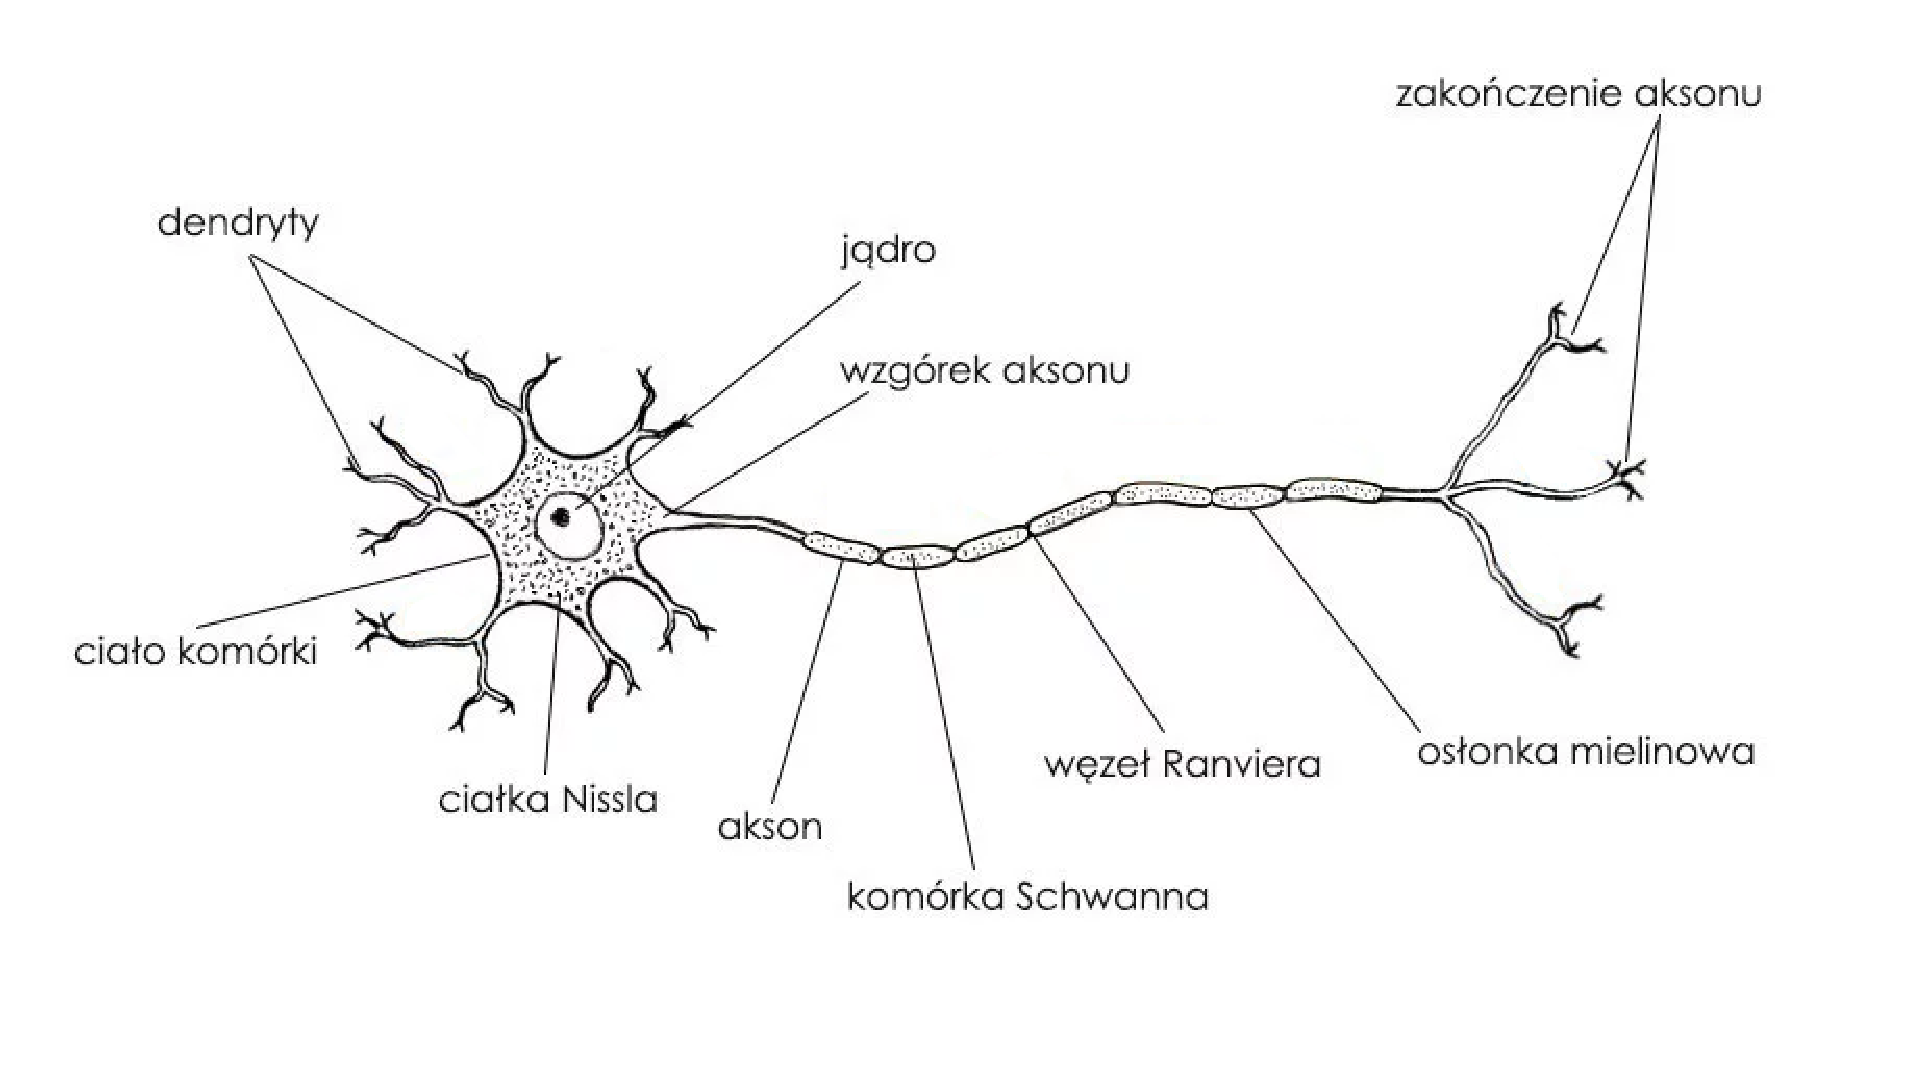
\includegraphics[width=\textwidth]{figures/neuron}
	\caption{Komórka nerwowa \tiny{źródło: www.fizjoterapeuty.pl}}
\end{figure}
Jak pokazano na rysunku \ref{fig:neuron} w skład komórki nerwowej wchodzą dendryty które zbierają
sygnały i akson który je przekazuje dalej.

\FloatBarrier
%--------------------------------------------------------------------------------------------------
\subsection{Model neuronu jako klasyfikator}

%--------------------------------------------------------------------------------------------------
\subsection{Uczenie sztucznych sieci neuronowych}

%--------------------------------------------------------------------------------------------------
\subsection{Konwolucyjne sieci neuronowe}


%==================================================================================================
\section{Architektura kontowlucyjna w detekcji chorób liścia kukurydzy}

\nocite{*}
\bibliography{bibliografia} 

\end{document}


